\documentclass[12pt]{beamer}
\usepackage[withmath]{uglibeamer2} %[withmath,withtikz]
\title{Deux activités en lien avec la cybersécurité}
\subtitle{NSI}
\author{}
\begin{document}
\maketitle


\begin{frame}[standout]
    \begin{center}
        \Huge
        Sécurisation des communications\\
        NSI1
    \end{center}
\end{frame}

\begin{frame}{Contenu}\pause

\textbf{But : } Faire constater aux élèves ce qui est effectivement transmis au serveur lors de la validation d'un formulaire comportant des données sensibles.\pause\\

\textbf{Lien avec le cours : } Complètement en phase avec le volet IHM de première.\pause

\textbf{Partie technique : } Du HTML et du Javascript, très simple, une fonction de hachage est exposée \textit{pour s'en servir}.\\\pause
Un travail d'observation des fonctions de hachage peut être fait avec la librairie standard de Python.

\end{frame}
\begin{frame}[fragile]
\begin{minted}[fontsize=\scriptsize,breaklines=true]{javascript}
    function validateForm() {
let x = document.forms["myForm"]["fPassword"].value; // On récupère la valeur de "fPassword"

if (x.match("^(?=.*[a-z])(?=.*[A-Z])(?=.*[0-9])(?=.*[ -/:-@\[-`{-~]).{8,16}$") == null)

    // la ligne du dessus verifie ci cette valeur correspond bien au motif désiré (voir plus bas)
{
    alert("Le mot de passe doit contenir une minuscule, une majuscule, un chiffre, un caractère spécial et " +
        "comporter entre 8 et 16 caractères.");
    document.forms["myForm"]["fPassword"].value = ""; // On vide le champ fPassword
    return false;
}
document.forms["myForm"]["fPassword"].value = SHA256(x); // Si le mot de passe est valable, on ne l'envoie pas
// on envoie son hash...
}
\end{minted}
\end{frame}

\begin{frame}
    Le code de la fonction SHA256 figure après le code ci-dessus, pour observation par l'élève.\pause


\begin{center}
    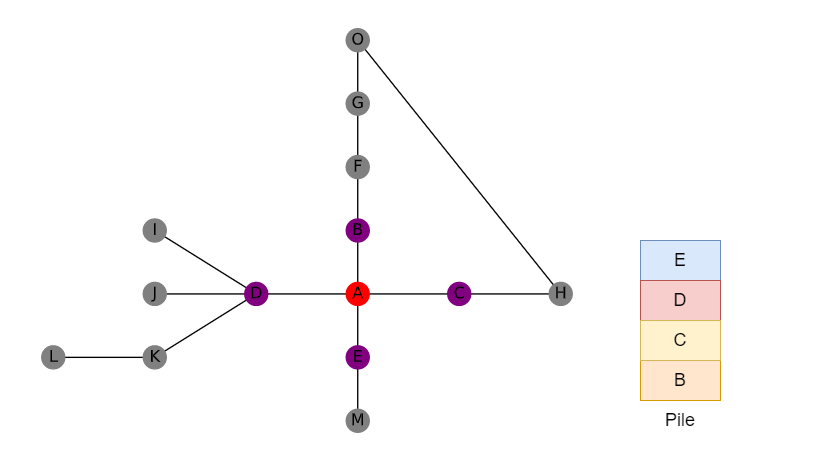
\includegraphics[width=5cm]{img/01.png}\\
    On valide le mot de passe...\\[2em]\pause@

    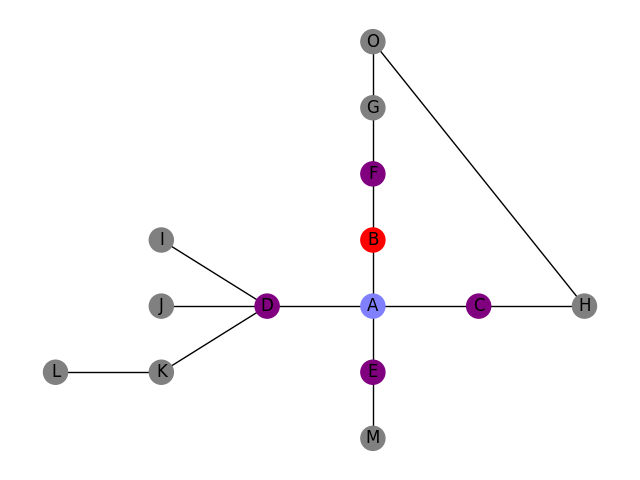
\includegraphics[width=\linewidth]{img/02.png}\\
    C'est son empreinte qui est transmise.

\end{center}

\end{frame}
\begin{frame}[standout]
    \begin{center}
        \Huge
        Sécurisation des communications\\
        NSI2
    \end{center}
\end{frame}


\begin{frame}{Contenu}\pause
\textbf{But :} Faire connaître et utiliser les algorithmes de chiffrements.\pause\\

\textbf{Lien avec le cours :} On fait comme le protocole HTTPS : une donnée est encryptées avec AES (encryptage symétrique), la clé de cryptage est encodée en RSA.\pause\\

\textbf{Partie technique :}\pause
\begin{itemize}
    \item utilisation de bibliothèques de cryptographie ;\pause
    \item on peut expliquer les algorithmes \textit{sans les prouver} ;
    \item les élèves peuvent créer une petite UI.\pause
\end{itemize}
\end{frame}

\begin{frame}
    \begin{center}
        \includegraphics[width=5cm]{img/seQre.png}\\

        Interface minimaliste créée avec \texttt{flet}.
        \end{center}     
\end{frame}


\begin{frame}[standout]
    \begin{center}
        \Huge
        D'autres pistes ?\\
    \end{center}
\end{frame}


\begin{frame}{Autres pistes}\pause
    \begin{itemize}
        \item Travail en première sur les critères de sécurité d'un mot de passe.
        \item Est-ce que c'est possible de faire un fil rouge ?
        \item Explorer autour des cookies.
        \item l'homme du milieu.
        \item les certificats ?
    \end{itemize}
\end{frame}
% RGS pour cookies
% PSSI pour se former (long)

% Chiffrer ou certifier est la réponse à l'homme du milieu ?
% Man in the middle en débranché ?
\end{document}
